Building upon the discussion of Kotlin's integration into Android development, it is crucial to contextualize this transition by considering the origins and foundational concepts of the fundamental programming languages and frameworks in use today. To this end, we shall delve into the historical development of Kotlin, Java, and Flutter. Each of these technologies has uniquely contributed to the evolution of software development practices and choices available to mobile developers. A brief exploration of their inception and initial objectives will provide valuable insights into their current roles and capabilities within the technology landscape.
\subsection{Java}
Java was developed in 1995 by Sun Microsystems, with the initial release being Java 1.0. It was designed by James Gosling and his team as a programming language that could run on any device without recompilation, known as "write once, run anywhere" \cite{raffles1817history}. Java's structure is based on classes and objects, following the object-oriented programming paradigm. It is a statically typed language, meaning variables must be declared before they can be used, enhancing code reliability and maintainability \cite{pinto2015large}. 
\par
Java is widely used for Android app development due to its portability, security features, and extensive standard library. Android apps are primarily developed in Java, making it the de facto language for Android development \cite{li2016accessing}. The Android Software Development Kit (SDK) provides developers with tools to build apps efficiently, leveraging Java's robust features. Additionally, Java's platform independence allows Android apps to run on various devices with different hardware and software configurations, contributing to its popularity in the mobile app development industry \cite{li2016accessing}.
\par
In the context of Android, Java is utilized to access Android APIs, enabling developers to interact with the underlying operating system and create feature-rich applications \cite{li2016accessing}. The structure of Java facilitates the development of complex Android apps by providing a well-defined syntax, memory management through garbage collection, and support for multithreading, which is essential for responsive and interactive mobile applications \cite{pinto2015large}.
\subsection{Kotlin}
Kotlin, a statically typed programming language supporting object-oriented and functional programming, was developed in 2011 by JetBrains. Inspired by various languages like Groovy, Kotlin aimed to address the limitations of existing languages and provide enhanced features for developers \cite{king2020history}. Kotlin's structure is designed to be concise and expressive, offering features like improved conditional execution with the "when" structure, which allows for more optimal handling of business tasks. Additionally, Kotlin incorporates modern language features such as null-safe navigation and coroutines for asynchronous programming \cite{li2022mapping}. 
\par
Kotlin is widely used for Android app development due to its interoperability with Java, seamless integration with Android Studio, and concise syntax, which increase developer productivity \cite{li2022mapping}. The language's versatility and compatibility with existing Java codebases make it a popular choice for building Android applications. Furthermore, Kotlin's safety features, such as null safety and immutability by default, contribute to writing robust and bug-free code.
\par
In Android development, Kotlin provides developers with tools like the Kotlin Coroutines library for asynchronous programming and the Gradle Kotlin DSL for project assembly, enhancing the development process \cite{king2020history}. Its concise syntax and modern features enable developers to create efficient and maintainable Android applications \cite{kartinah2023android}. Kotlin's popularity in Android development is further evidenced by its use in various research projects focusing on Android-based applications. 
\subsection{Dart(Flutter)}
Flutter is a versatile app SDK developed by Google that allows developers to create high-performance applications for various platforms like iOS, Android, and the web using a single codebase \cite{bouchemal2020scream}. It was initially released in 2017 and has gained popularity due to its ability to provide a consistent user experience across different platforms. 
\par
Flutter's architecture is based on the Dart programming language, which Google also developed. Dart is an object-oriented, class-based language that supports interfaces, mixins, abstract classes, and optional typing. It is optimized for building user interfaces and allows for ahead-of-time compilation of native code for better performance \cite{ernawati2021android}.
\par
Flutter uses a reactive framework composed of widgets, which are the building blocks of Flutter applications. Widgets in Flutter are arranged hierarchically to create the user interface. Flutter's architecture allows for hot reload, which enables developers to see the changes they make to the code reflected in the app almost instantly, making the development process more efficient \cite{pratama2021pengembangan}.
\par
One of the critical reasons why Flutter is used is its ability to create cross-platform applications with a single codebase. This significantly reduces development time and effort as developers do not have to write separate code for different platforms. Additionally, Flutter provides a rich set of customizable widgets, a fast development cycle, and strong community support, making it an attractive choice for developers \cite{pratama2021pengembangan}.
\subsection{Previous Research}
\subsubsection*{Kotlin's Transition and Adoption in Android Development}
The transition from Java to Kotlin in Android development is motivated by Kotlin's advanced features like null safety, extension functions, and concise syntax, which collectively enhance code readability and maintainability. Kotlin's interoperability with Java and official support by Google further drive its adoption despite challenges related to the learning curve and migration efforts \cite{hegedHus2022static}. On the other hand, Flutter's emergence as a cross-platform framework offers the advantage of natively compiled applications from a single codebase across various platforms, supported by its widget-based architecture and the Dart programming language \cite{mazuera2022taxonomy}. However, concerns persist regarding Flutter's performance compared to native applications and the maturity of its ecosystem.
\par
Recent research by V. Oliveira, L. Teixeira and F. Ebert. \cite{oliveira2020adoption} explores the adoption of Kotlin for Android development through a mixed-methods approach, combining quantitative analysis of Stack Overflow discussions with qualitative interviews of Android developers. This study highlights the rapid acceptance of Kotlin following its endorsement by Google, attributing its popularity to features like null safety, expressiveness, and interoperability with Java. These attributes have facilitated a smoother transition for developers migrating from Java, enabling them to utilize existing Java libraries while benefiting from Kotlin's modern features.
\par
Developers appreciate Kotlin's concise syntax and enhanced safety features \cite{oliveira2020adoption}, contributing to more robust and maintainable code. However, the study also reveals challenges, such as the complexity introduced by Kotlin’s functional programming capabilities, which some developers find obscure and challenging to manage in larger codebases. Interoperability with Java, while largely beneficial, introduces its complexities, mainly when dealing with nullability and Java's legacy code.
\par
To determine the effect of code smells on software maintainability, Matheus Flauzino conducted an empirical analysis of the prevalence of code smells in Java and Kotlin, examining more than 6 million lines of code from 100 GitHub repositories. This paper is essential for developers debating whether to use Java or Kotlin since it shows conclusively that the latter tends to have fewer code smells, which is a surefire sign of future maintenance issues. The study analyzed five prevalent code smells and found that Kotlin consistently displays fewer examples of these troublesome patterns except for the Long Parameter List than Java. The results imply that Kotlin's design, which prioritizes readability and conciseness, may naturally prevent code smells from developing. Because of this, Flauzino et al.'s paper highlights the complex factors in selecting a programming language for software development and presents a strong case for using Kotlin over Java for projects where maintainability is a concern \cite{flauzino2018you}. 

\subsubsection*{Improving Code Quality and Software Maintenance}
The focus on code quality in mobile app development, including integrating tools like SonarQube, emphasizes the importance of managing technical debt and addressing code smells \cite{hecht2015detecting}. Innovations like ecoCode emphasize energy-efficient coding practices, reflecting a broader concern for sustainable software development. Comparative studies on development methodologies provide insights into the challenges and considerations involved in transitioning between frameworks, offering valuable practical experiences for developer \cite{lamothe2020a3}.
\par
Evaluating open-source projects offers practical insights into applying different development methodologies, aiding in identifying patterns, best practices, and common pitfalls associated with various programming languages and frameworks. Despite the wealth of knowledge on mobile app development frameworks, there is a gap in research that combines practical development experience with a thorough analysis of open-source projects across diverse frameworks, particularly in exploring the effects of methodologies on code quality metrics like code smells and their severity \cite{ardito2020effectiveness}.
\par
The prediction of code smells in continuous integration is a critical task for quality managers and developers. A recent study by Md Abdullah Al Mamun \cite{mamunimproving} investigated the effectiveness of organic versus cumulative software metrics in predicting code smells. The researchers used over 36,000 software revisions from 242 open-source Java projects to develop predictive models. Their findings revealed that non-cumulative (organic) metrics, which reflect changes between revisions rather than aggregated totals, were significantly more effective in predicting code smells. This is because organic metrics are more sensitive to recent changes in code, offering a more accurate measure for predicting software quality issues.
\par
In contrast, cumulative metrics were less effective, potentially masking recent developments that were more indicative of current software quality. The distinction between organic and cumulative metrics is essential for quality managers and developers in continuous integration environments, where quick iterations and timely quality assessments are crucial. The study also employed various model validation techniques to ensure the generalizability of the results.

\subsubsection*{Static Analysis Tools and Their Application}
Static analysis tools have been recognized as valuable for improving software quality. However, a recent study by D. Marcilio \cite{marcilio2019static} critically examined SonarQube, a leading static analysis tool, in real-world software projects across various organizational settings, including open-source communities and government institutions. The study revealed that despite the perceived effectiveness of static analysis tools in enforcing coding standards and reducing technical debt, the actual resolution rate of identified issues remains low, with an average resolution rate of only 13% across the studied projects. While problems are typically fixed within about 19 days of being reported, the low overall resolution rate suggests that many issues identified by SonarQube need to be prioritized or deemed non-critical by developers. Moreover, the customization of SonarQube instances in different organizations led to significant variance in the types of issues that are reported and addressed, with some organizations using highly customized configurations that may not effectively capture the most critical violations or could lead to a high number of false positives, further complicating the developers' decision-making process regarding which issues to address.
\par
The study conducted by Ifeanyi Rowland Onyenweaku \cite{onyenweaku2021sonarqube} aimed to evaluate the effectiveness of static analysis tools in identifying defects in software applications, with a focus on the use of SonarQube in analyzing Spectral Workbench, a tool used for capturing and analyzing spectral data. The researchers found that SonarQube successfully identified many defects, ranging from minor UI issues to critical bugs, which could cause system failures if not addressed. Their analysis revealed 232 code smells and 63 bugs, providing a detailed categorization of issues by severity and type, which could aid developers in prioritizing which issues to address first. The study also highlighted the challenge of low-resolution rates for identified issues in software development, with constraints such as prioritization, resource allocation, and perceived severity often playing a role. Despite this, the researchers emphasized the potential of integrating SonarQube into open-source projects, providing a blueprint for other projects. Overall, the findings of this study demonstrate the value of static analysis tools in enhancing the reliability and effectiveness of software applications while highlighting the challenges that need to be addressed to improve the resolution rate of identified issues.
\par
The research conducted by Sebastian Stiernborg on the application of SonarQube in the open-source project Spectral Workbench has been instrumental in providing a deeper understanding of the practical usage of this tool in a corporate setting. The study presents a comprehensive view of the operational challenges and benefits associated with implementing continuous inspection processes, thereby contributing to the body of knowledge in this domain. In his master thesis \cite{stiernborg2019automated}, Sebastian Stiernborg delves into the efficacy of implementing continuous inspection processes within software development teams, specifically focusing on SonarQube. The study was conducted in collaboration with Furhat Robotics' development team, where Stiernborg worked closely to introduce SonarQube to their existing development processes. The primary objective of the integration was to automate code reviews and improve code quality without disrupting the developers' workflow. The study presents a set of guidelines based on feedback from integrating continuous inspection tools, highlighting the advantages of such tools, including the early detection of defects and enhanced code quality. However, the study also identifies potential challenges, such as the complexity of integrating these tools within existing systems and the need for careful handling to avoid disruption and ensure developer buy-in.
\par
Furthermore, Stiernborg's research emphasizes the need for further studies to explore the integration of different continuous inspection tools and features. One of the key findings from the research is the challenge of balancing the immediate benefits of continuous inspection with the initial resistance and learning curve associated with adopting new tools. The study details the specific implementation steps taken at Furhat Robotics, including the challenges of configuring and maintaining such tools within existing systems and the strategies employed to overcome these challenges. Overall, the study contributes to the growing body of research on continuous inspection processes and highlights the importance of careful planning, implementation, and evaluation of such tools in software development teams.
\par
The study conducted by Sebastian Stiernborg \cite{stiernborg2019automated} on integrating static analysis tools and its impacts on maintenance activities was further enriched by Ze ́phyrin Soh's \cite{soh2016code} investigation. Soh's study quantified the specific effects of code smells on various maintenance tasks, offering a more detailed perspective on the implications of code quality on software maintainability. Soh's research is particularly noteworthy as it differentiates between different types of maintenance efforts, such as editing, navigating, reading, and searching, unlike previous studies that treated maintenance effort as a monolithic activity. The study revealed that code smells have varying impacts on different maintenance activities. While some code smells may increase the effort required for tasks such as navigating and editing, they do not uniformly affect all maintenance activities. For instance, the code smell "Feature Envy" significantly increased the effort required for searching activities, whereas "Data Clumps" primarily elevated the effort in editing tasks. This nuanced view provides a more granular understanding of developers' practical challenges when dealing with code smells in a maintenance context. The study also utilized a sophisticated methodological approach, utilizing multiple linear regressions to analyze the impact of code smells while considering other factors such as file size and number of revisions. This approach validates the significant role of code smells in increasing maintenance effort and refines our understanding of their impact relative to other factors such as file size and changes made.
\par
Ensuring high-quality code is fundamental to developing effective and efficient software engineering software. However, recent research \cite{corral2015better} conducted by Corral and Fronza challenges the notion that superior code quality is the primary determinant of app success in the Google Play store. The study examined the relationship between source code quality and market success indicators, such as the number of downloads and user ratings, using a sample of 100 open-source mobile applications. Results revealed a relatively marginal impact of source code quality on market success indicators, suggesting that factors such as marketing strategies, app functionality, user interface design, and overall user experience play more significant roles in determining the success of mobile applications in app stores. The methodology employed by Corral and Fronza involved using statistical methods to establish a strong correlation between established source code metrics and app store success metrics. The findings underscore the complexity of app success and highlight the limitations of relying solely on technical excellence in a market driven by consumer preferences and competitive features \cite{corral2015better}. In the research conducted by Luis Corral and Ilenia Fronza, Figure \ref*{fig:graph_lr} showcases a visual representation of the market success model based on app store metrics such as Number of Downloads (NOD), Number of Reviewers (NOR), and Application Rating (AR). This figure effectively demonstrates how these metrics collectively contribute to defining the market success of mobile applications. NOD measures the popularity and reach of an app by indicating how many times it has been downloaded, thus indirectly measuring its visibility and user interest. NOR, on the other hand, represents users' engagement with the app by counting how many users have taken the time to review it. Lastly, AR, which is averaged from all user ratings, offers a direct insight into user satisfaction and perceived app quality. Combined, these metrics provide a comprehensive view of an app's performance in the market. They portray how often it was downloaded, how well users received it, and the extent of active user interaction and satisfaction.
\begin{figure}[htbp]
    \centering
    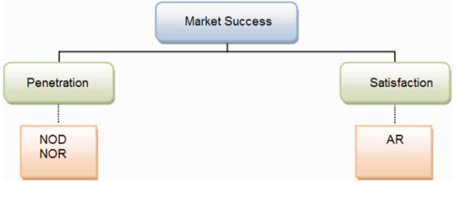
\includegraphics[scale = 0.8]{img/graph_lr.png}
    \caption{Corral and Fronza's research resulted in a Market Success Model Based on App Store Metrics.}
    \label{fig:graph_lr}
\end{figure}

The study by Michele Tufano \cite{alkhaeir2020effect} sheds light on the origins and persistence of code smells in significant software ecosystems, presenting critical insights into the internal software development processes. The empirical analysis conducted on 200 open-source projects from Android, Apache, and Eclipse ecosystems traces the history of code changes to pinpoint when specific code smells are introduced and under what conditions they are most likely to occur. The study \cite{alkhaeir2020effect} finds that many smells are introduced at the inception of code entities or through changes that do not directly relate to ongoing maintenance, challenging the prevailing assumption that code smells primarily emerge during routine maintenance and evolution activities. The research used a metric-based methodology to detect smell-induced changes, providing a granular view of how smells develop over time. The findings suggest that tool-based smell detection and refactoring recommendations should consider the specific developmental context to be truly effective and advocate for the development of more sophisticated recommendation systems that could help developers plan and implement refactoring activities more strategically, thereby potentially reducing the introduction of new smells during both development and maintenance phases.
\par
Building on Michele Tufano's analysis \cite{tufano2015and} of the origins of code smells, the research \cite{alkhaeir2020effect} conducted by Tarek Alkhaeir and Bartosz Walter sheds further light on the significant impact these smells have on the relationship between design patterns and defects. Their study \cite{alkhaeir2020effect} highlights that code smells can significantly exacerbate the likelihood of defects in software projects where design patterns are implemented. Through an analysis of Java classes from ten systems in the PROMISE dataset, Alkhaeir and Walter critically evaluate how design patterns and code smells correlate with increased defects. Their work confirms that classes utilizing design patterns are not inherently defect-prone but become so when code smells are present. The study establishes a clear connection between smelly and non-smelly design pattern classes and defects using statistical tests. The findings indicate that pattern classes with code smells experience more defects than their non-smelly counterparts, underscoring the substantial negative impact of code smells on software quality. The researchers also observed that while non-smelly design patterns tend to have a neutral or slightly negative effect on defect proneness, introducing code smells drastically increases the likelihood of defects.
\par
Xiaofeng Han and colleagues conducted a study \cite{han2021understanding} to explore the practical applications of code reviews in identifying and addressing code smells within the OpenStack community. Drawing on prior research on code smells in software systems, the study reveals that code smells are critical indicators of potential maintenance issues often overlooked during the review process. Specifically, the researchers examined code reviews within the Nova and Neutron projects and found that coding convention violations or oversights by developers were common causes of code smells. However, when code smells were identified, reviewers provided actionable recommendations for refactoring, typically implemented by developers, improving code quality.  The study highlights the value of manual code review over automated tools, as the former is more context-sensitive and effective in identifying subtle issues. The researchers found that enhancing the code review process with better guidelines and training on smell detection could further improve the effectiveness of this quality assurance practice. This collaborative approach to code review reinforces the importance of adhering to coding standards and demonstrates that code reviews are crucial to identifying and addressing code smells despite the challenges involved.




\subsubsection*{Emergence and Impact of Flutter in Cross-Platform Development}
Cross-platform development tools, including Flutter, are rapidly transforming the landscape of mobile application development by offering significant reductions in code complexity and enhancing maintainability—a study by \cite{cheon2021converting}.	Y. Cheon and C. Chavez demonstrated that when an existing Android application was rewritten in Flutter, it could run on Android and iOS platforms and required approximately 37\% fewer lines of code than the original Java implementation \cite{cheon2021converting}. This reduction is primarily attributed to Flutter's streamlined approach to UI development and robust widget library, which significantly diminishes the need for verbose UI code and extensive platform-specific adaptations.
\par
Furthermore, the transition from Java to Flutter revealed that Flutter's declarative UI framework and reactive programming model could improve application performance and responsiveness. By moving away from the imperative and stateful approaches typical in Android development, Flutter enables more dynamic and efficient handling of UI changes, leading to smoother user experiences \cite{nawrocki2021comparison} This shift is crucial for developers looking to build highly interactive and responsive applications without the overhead of managing complex state synchronization across user interface components. 
\par
The triangulation method used in the study—analyzing discourse from Stack Overflow alongside direct developer interviews—provides a comprehensive understanding of the practical challenges and benefits developers observe in real-world scenarios. This approach confirms the theoretical advantages of Kotlin discussed in previous literature and illuminates the nuanced difficulties encountered during its practical application.
\par
The evolution of programming languages like Java and Kotlin and frameworks such as Flutter has significantly shaped the landscape of Android application development. Each technology brings unique strengths for mobile app creation, from Java's "write once, run anywhere" principle to Kotlin's modern syntactic features and Flutter's cross-platform capabilities. This diversity allows developers to select technologies that best fit their project's requirements and personal or team proficiency. However, as the technology landscape continuously evolves, developers must remain adaptable, continually updating their skills and understanding of these tools. The ongoing transition towards more efficient, readable, and maintainable coding practices suggests a promising future for mobile development. By embracing these changes and learning from comparative and empirical studies, developers can better navigate the complexities of modern app development, ensuring robust, efficient, and user-friendly applications.
